\documentclass[12pt]{article}

\title{An axiomatic review of anisotropic quantum gravity}
\author{S. Halayka\footnote{sjhalayka@gmail.com}}
\date{\today\;\currenttime}

\usepackage{datetime}
\usepackage{listings}
\usepackage{cite}
\usepackage{xcolor}
\usepackage{graphicx}
\usepackage{setspace}
\usepackage{amsmath}
\usepackage{url}
\usepackage[margin=0.8in]{geometry}
%\usepackage{comment}
%\doublespace

\usepackage{xcolor,colortbl}

\newcommand{\mc}[2]{\multicolumn{#1}{c}{#2}}
\definecolor{Gray}{gray}{0.9}






\begin{document}



 
\maketitle



Shawn Halayka

741 McCraney Crescent

Prince Albert, SK Canada

S6V 6W3



\begin{abstract}
In Newton's and Einstein's theory, all mass gravitates in an {\textit{isotropic}} (spherical) manner.
In this paper, we will consider {\textit{anisotropic}} gravitating processes.
We discuss dark matter, as well as dark energy and the possibility of a final, $5$th interaction.
We provide a numerical solution in C++.
\end{abstract}


\section{Questions}

In this paper we will address the following three questions:
\begin{enumerate}
\item The hierarchy problem: why is gravitation so weak?
\item The dark matter problem: why is gravitation stronger than that predicted by general relativity in pressure-free dusts such as the Galactic disc?
\item The dark energy problem: why is the Universe undergoing accelerating expansion?
\end{enumerate}






\section{Axioms}

Here we provide a list of $11$ axioms regarding relativity:

\begin{enumerate}
\item Speed causes kinematic time dilation.
\item The gravitational field causes gravitational time dilation.
\item Physical processes are interruptible, and are indeed interrupted when undergoing time dilation.
\item Processes undergoing heavy kinematic time dilation are deflected twice as much as in Newtonian gravitation -- for neutrinos, there is (practically) no internal process occurring to resist the gravitational attraction.
\item Physical processes are computations.
This is not merely an analogy, it's reality.
\item Computations can be optimized, so there is time contraction and length dilation to consider.
\item The densest process for any given mass $M$ or entropy $S$ is a black hole -- they are the most optimal of computations.
\item The gravitational field is quantized into gravitons.
\item There is no gravitational shadow -- the relaying of gravitons is the cause of gravitational time dilation.
\item Gravitationally-bound, pressure-free dusts, such as the Galactic disc, have fractional dimension. As the dimension reduces, the strength of the gravitation increases -- the dimension reduces as the shape of the Milky Way goes from spherical to disc-like with distance from the Galactic centre.
\item The self-optimization of the Universal process over time leads to length dilation, in the form of expansion -- the antithesis of attractive gravitation.
\end{enumerate}







\section{Results}

We have constructed Table 1 by first taking into account the inherent 3-D nature of isotropic gravitation, and its 4-D communications (e.g. {\textit{the}} Wilson hypervolume).
Next, we extrapolate all the way down, to where the strong interaction is 2-D, with 1-D communications (e.g. some Wilson lines). 
Finally, the possibility of a 5th interaction follows suit, in order to bring balance to the interactions in terms of their inherent spatial dimension.


\begin{table}
\caption{Table of interactions, including a 5th interaction.}
\begin{center}
\begin{tabular}{| l | r | r |}
  \hline
  Type & Inherent spatial dimension $D$ & Communication spatial dimension \\
\hline
\hline


Gravitation (isotropic) & 3  & 4\\

\rowcolor{Gray}
Gravitation (oblate) & 2 & 3\\

Gravitation (prolate) & 1 & 2\\

\rowcolor{Gray}
Weak & 0 & 1\\

Electromagnetism & 1 & 0 \\

\rowcolor{Gray}
Strong & 2 & 1\\

$5$th interaction & 3 & 2 \\
  \hline
\end{tabular}
\end{center}
\end{table}


Note that, unlike with the many Wilson lines per process, there is only one Wilson hypervolume, shared by all processes.
This means that gravitational interactions are {\textit{connectionless}} -- isotropic gravitation is {\textit{broadcast}}; there is no specific recipient (e.g. everyone is a target).
On the other hand, the strong interactions are more directed, and {\textit{connected}} -- strong interaction is {\textit{unicast}} or {\textit{multicast}}; there is a specific recipient (e.g. not everyone is a target).
For instance, the transition from broadcast transmission to directed transmission occurs as dark matter is factored in (e.g. where $D < 3$) -- see Figs. 1 and 2 for a simplified analytical solution for anisotropic gravitation in the Milky Way.
Connectedness is an attribute of the non-gravitational interactions (e.g. weak, electromagnetic, strong, and 5th interaction).







\section{Conclusion}

To answer the questions from the first section:
\begin{enumerate}
\item Why is gravitation so weak? 
Because it's often isotropic due to isotropic internal pressure.
\item Why is gravitation stronger than that predicted by general relativity in pressure-free dusts such as the Galactic disc? 
Fractional dimension and anisotropic gravitation.
\item Why is the Universe undergoing accelerating expansion? 
Accelerating Universal computational self-optimization.
\end{enumerate}









\section{Further questions}
\begin{itemize}
%\item Does the Universe have exactly three inherent spatial dimensions?
%If so, then is the Universe finite and closed (e.g. a 3-sphere in the Wilson hypervolume)?
\item Is a 5th interaction the same tetrahedral process that is predicted by (Wilson) loop quantum gravity?
If so, then are superstring theory and loop quantum gravity fundamentally compatible?
\item Do gravitons undergo Shapiro time delay?
If so, then are graviton condensates naturally cold?
\item Is a photon a gas of constituent particles related to a 5th interaction?
If so, are all particles made up of constituent particles related to a 5th interaction?
\item Can a human-scale object become pressure-free internally? 
If so, then does the gravitation become anisotropic as predicted in this paper?
\end{itemize}




\section{Numerical solution for anisotropic gravitation}

A copy of the C++ code for Figs. 3 through 7 can be obtained from:

\url{https://github.com/sjhalayka/ellipsoid_emitter}

This C++ code calculates an anisotropic gravitational field, and allows the coder to view the results using OpenGL or gnuplot.
For instance, Fig. 3 shows the intersection count (e.g. field strength) as the dimension of the gravitational field reduces from $D = 3.0$ to $D = 2.001$. 
Figs. 4 through 6 show an example gravitational field that goes from $D = 3.0$ to $D = 2.5$ to $D = 2.001$.
Figs. 7 through 9 show an analysis of the data -- the result is that $GM c^{3 - D}$ is a constant.





\begin{thebibliography}{9}

\bibitem{halayka} Halayka. Is the anisotropic interaction of luminous matter responsible for the extrinsic gravitation usually attributed to exotic dark matter? (2008)
\bibitem{halayka2} Halayka. A note on anisotropic quantum gravity. (2023)
\end{thebibliography}





\pagebreak


\begin{figure} 
\centering
  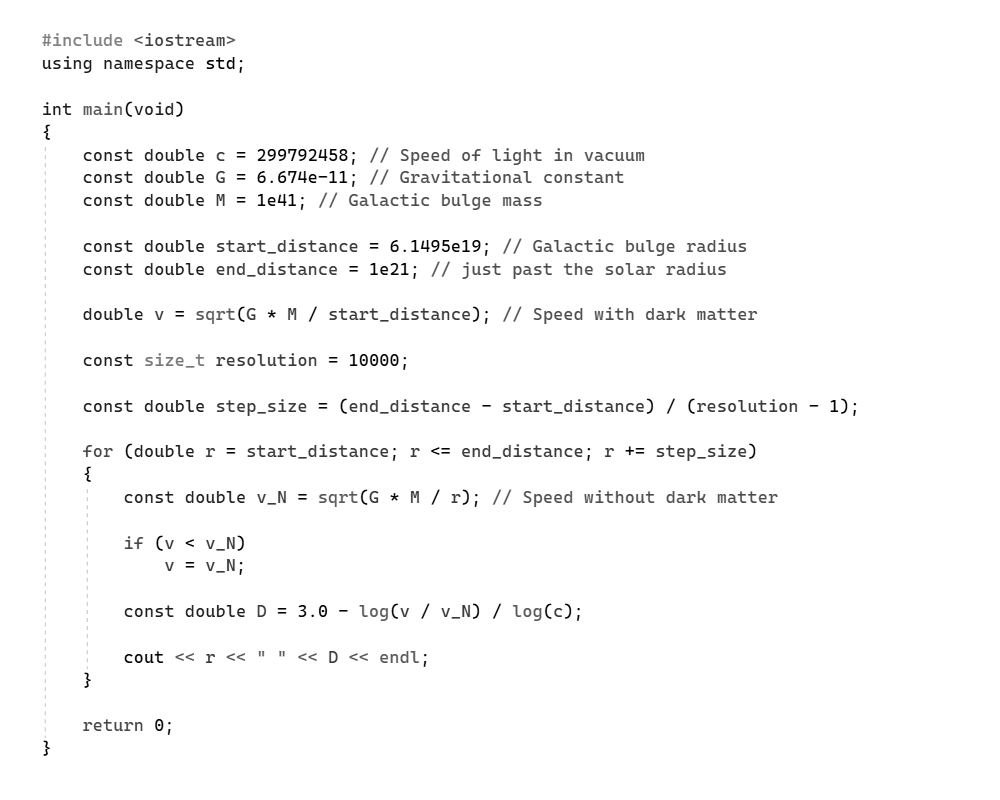
\includegraphics[width = 5 in]{code.png}
  \caption{ C++ code for Galactic orbit. 
Here $D$ represents dimension.
Note that where $D < 3$ that $D$ is the lower bound, and that the value of $D$ will actually be a little bit higher since the strength of the gravitation field increases {\textit{and}} falloff decreases as $D$ reduces.
In other words, the code does not take this small change in falloff into account, in order to keep things as simple as possible while still highlighting the role of fractional dimension.
}
\end{figure}


\begin{figure} 
\centering
  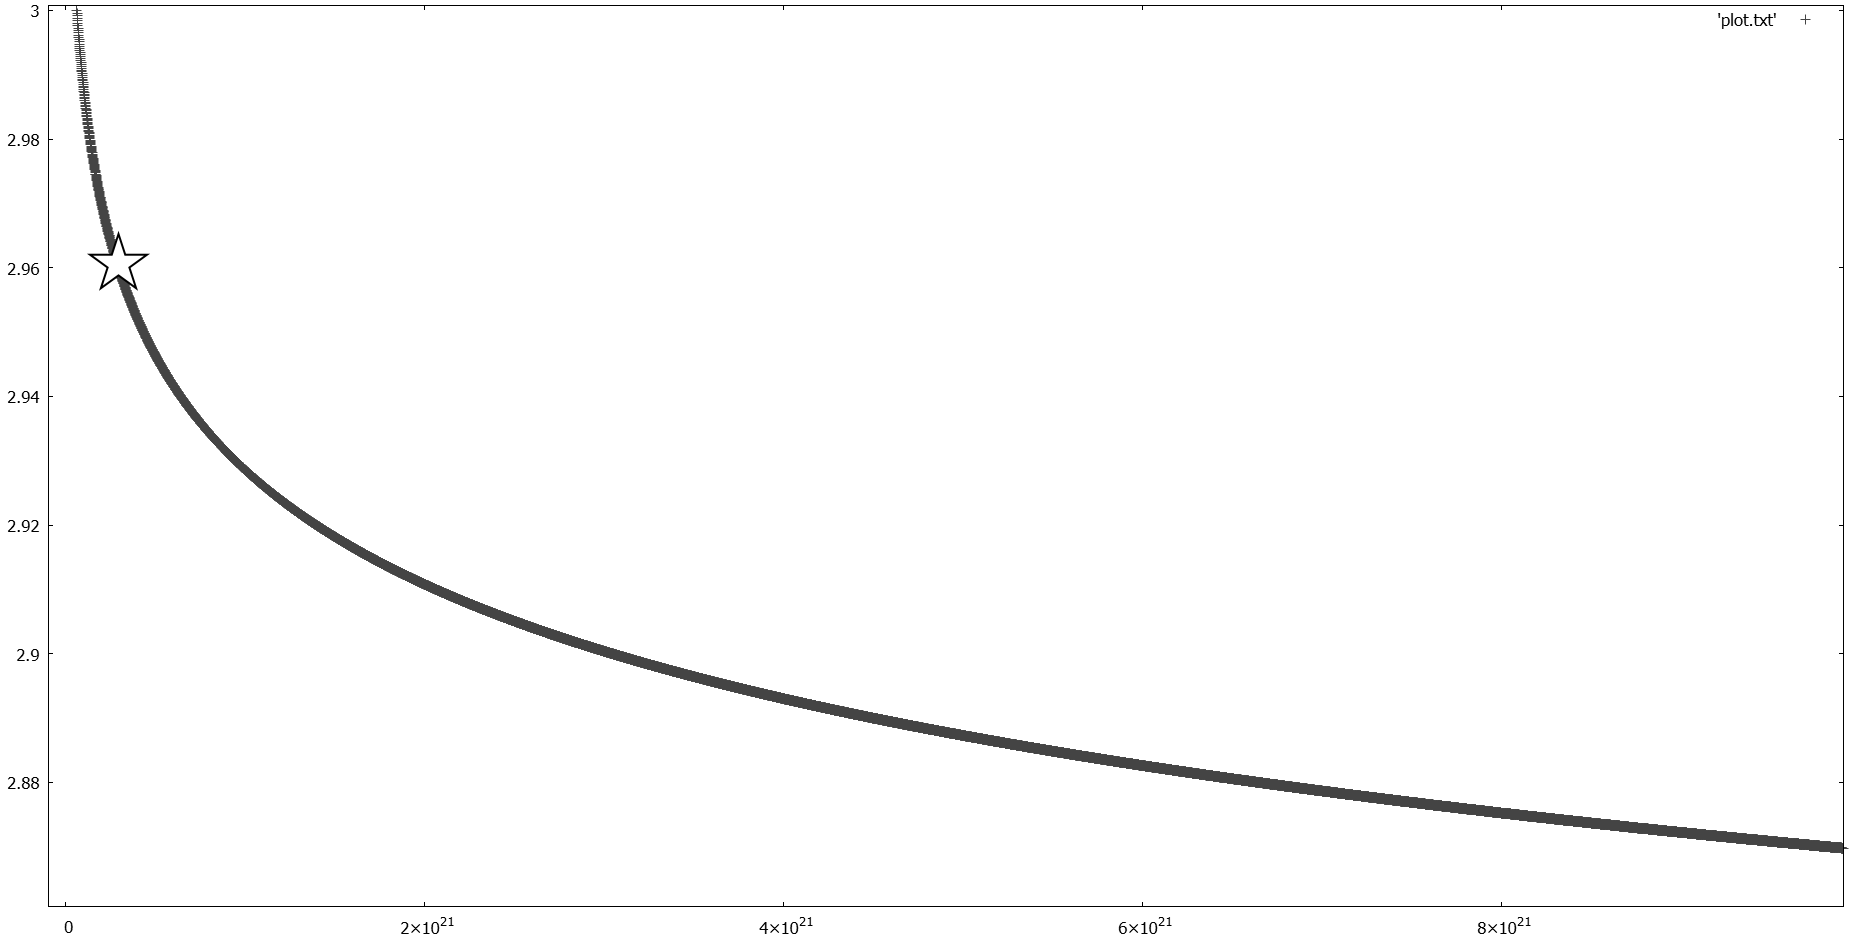
\includegraphics[width = 5 in]{dimension_graph.png}
  \caption{ Output from the C++ code in Fig 1.
Here the $x$ axis is the distance from the Galactic centre $r$, and the $y$ axis is dimension $D$.
Note that the lower bound is $D = 2.96$ at $r = 3 \times 10^{20}$ metres from the Galactic centre (e.g. the Solar orbit radius).
}
\end{figure}










\begin{figure} 
\centering
  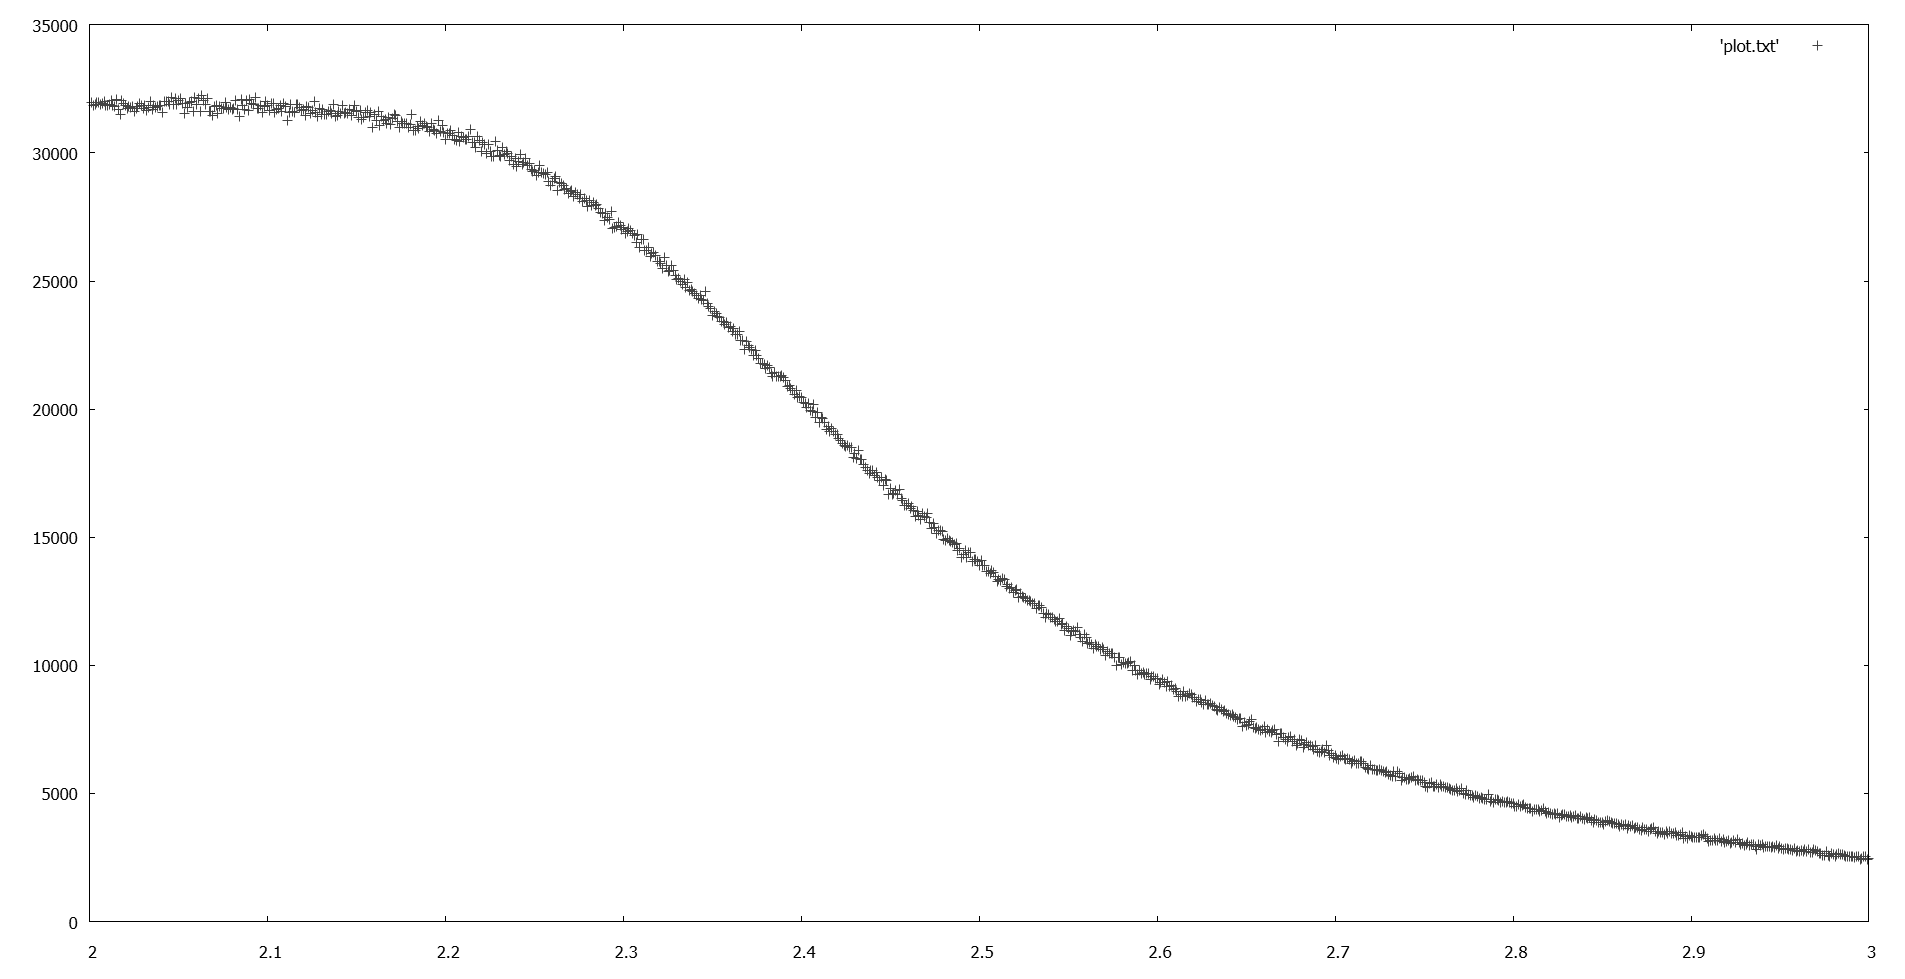
\includegraphics[width = 5 in]{transition.png}
  \caption{
Here the $x$ axis is dimension $D$, and the $y$ axis is intersection count (e.g. field strength).
It forms a nice sigmoid curve.
%Although not shown here, it is important to also note that falloff decreases from $1/r^2$ to $1/r^1$ as $D$ reduces from $3$ to $2$ -- see Figs. 4 through 6.
}
\end{figure}








\begin{figure} 
\centering
  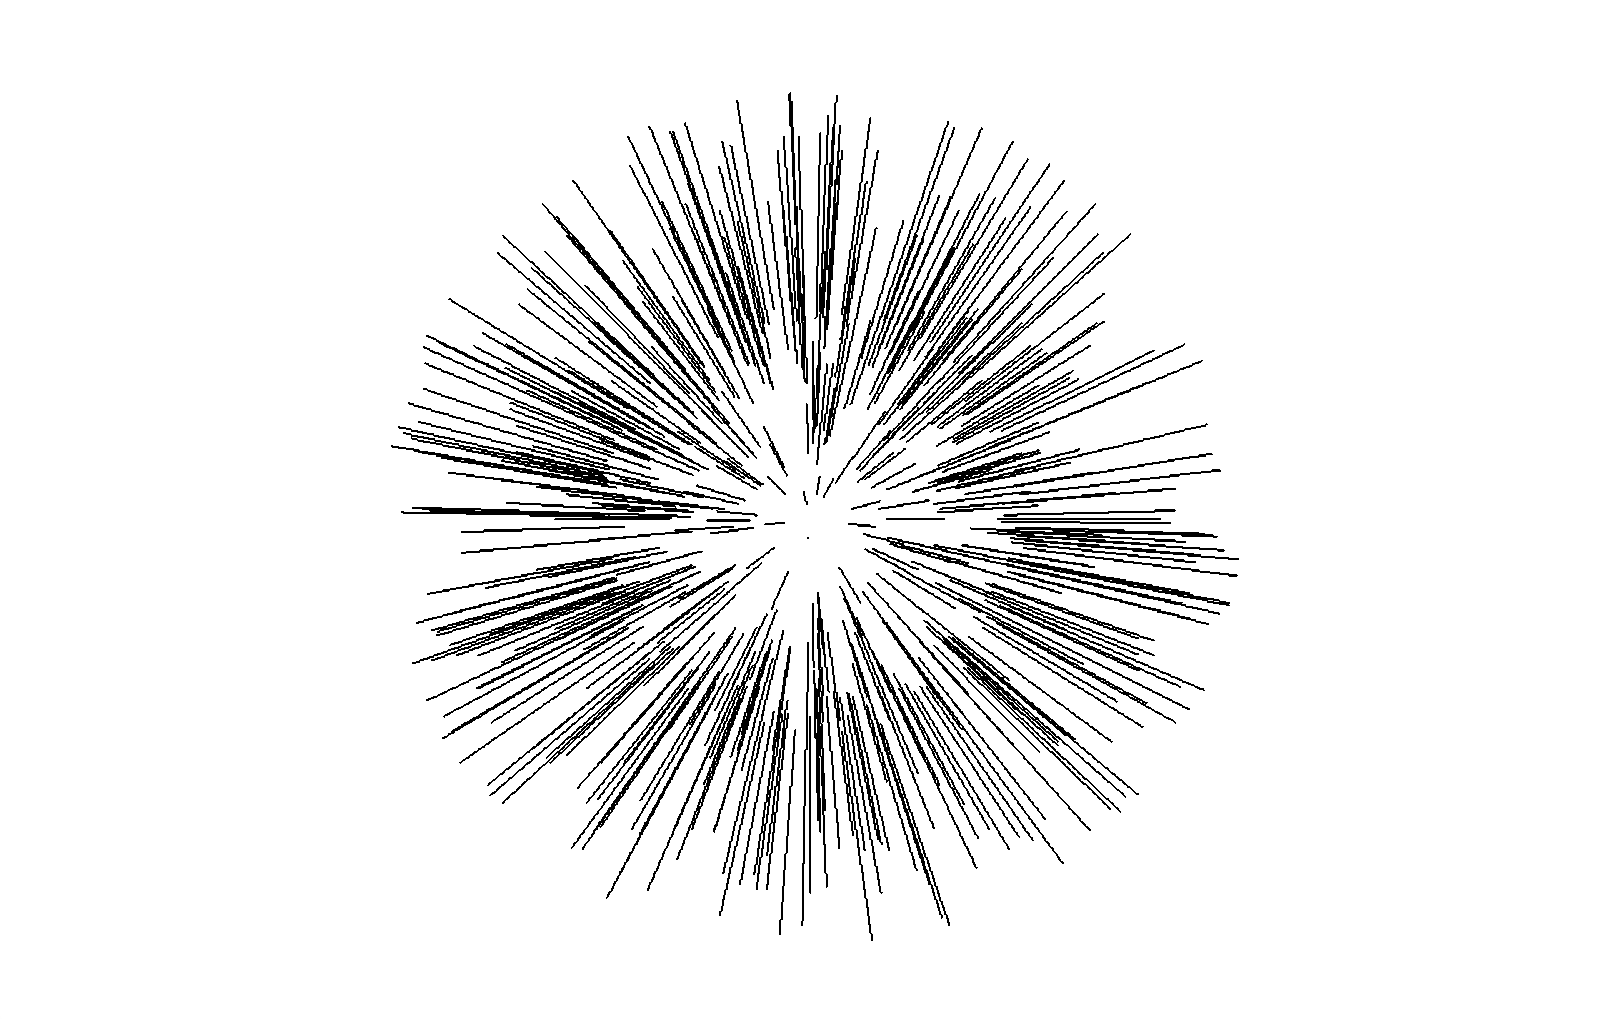
\includegraphics[width = 5 in]{3.png}
  \caption{
Example of an isotropic emitter.
Here $D = 3.0$. 
The emitter is spherical.
The positions are placed pseudorandomly on a 2-sphere, and the normals are calculated using the same sphere.
The strength of the gravitational field is $G$, and the intersection count gradient falloff is related to $1/r^3$ -- in other words, standard Newtonian gravitation.
}
\end{figure}


\begin{figure} 
\centering
  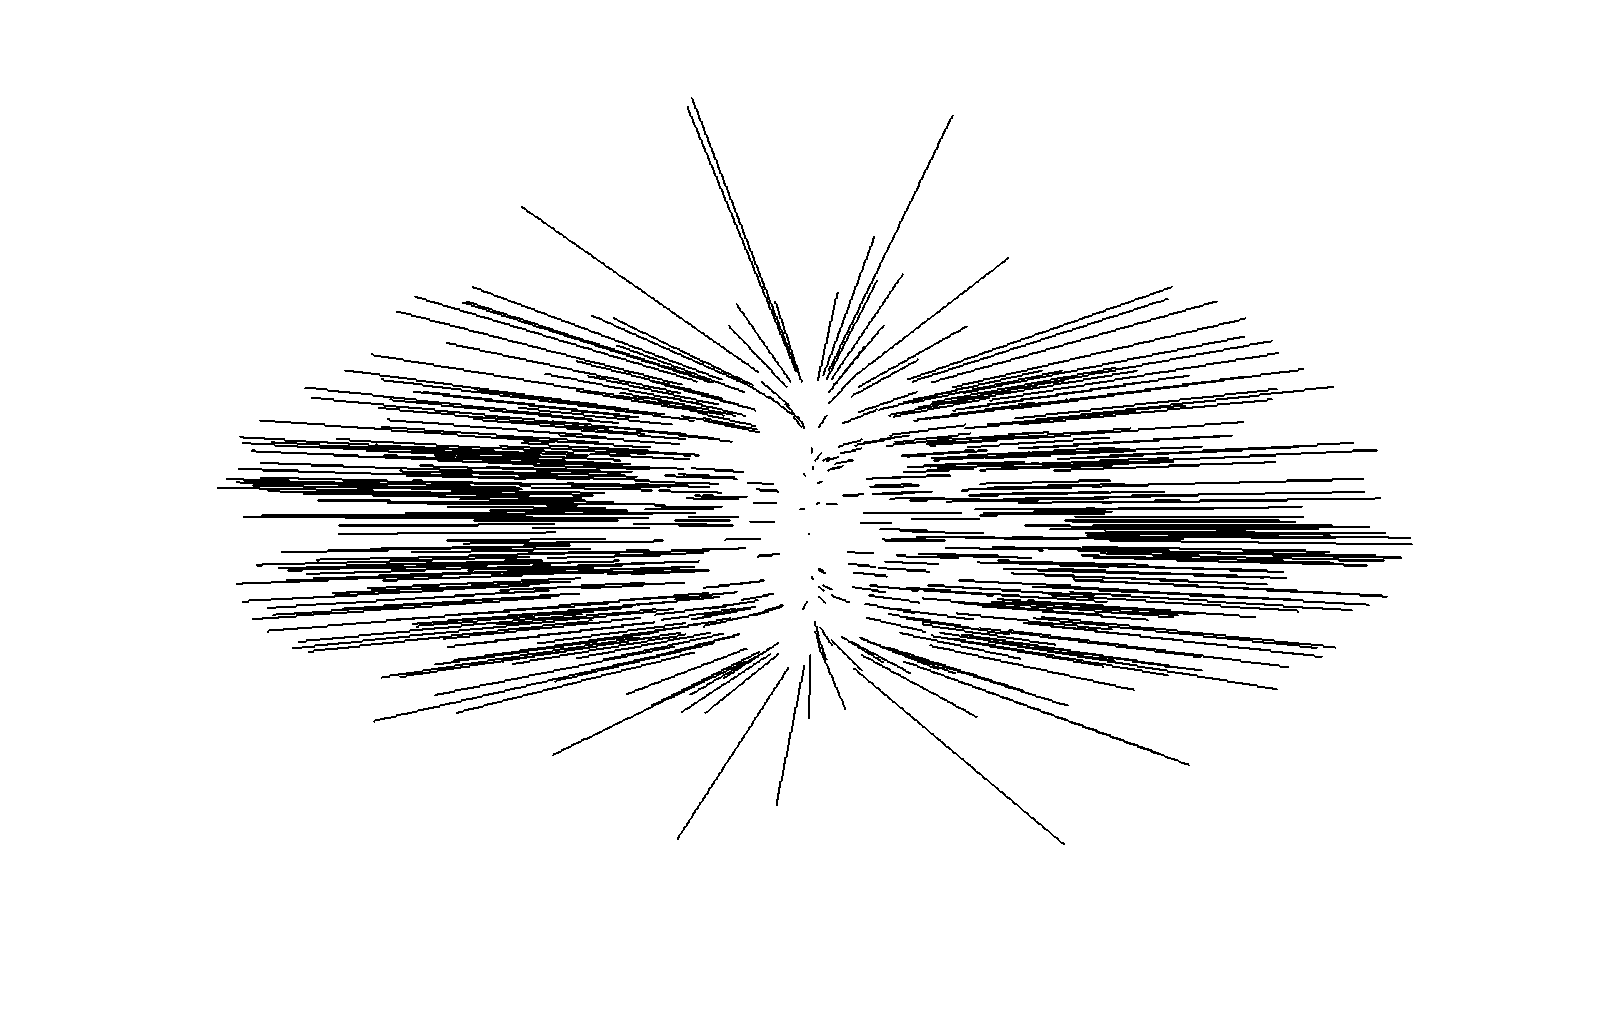
\includegraphics[width = 5 in]{2.5.png}
  \caption{
Example of an anisotropic emitter.
Here $D = 2.5$. 
The emitter is ellipsoidal.
The positions are placed on an oblate (e.g. flattened) ellipsoid, and the normals are calculated by using the dual prolate (e.g. tall) ellipsoid.
The strength of the gravitational field is like $G c^{0.5}$, and the intersection count gradient falloff is related to $1/r^{2.5}$.
}
\end{figure}


\begin{figure} 
\centering
  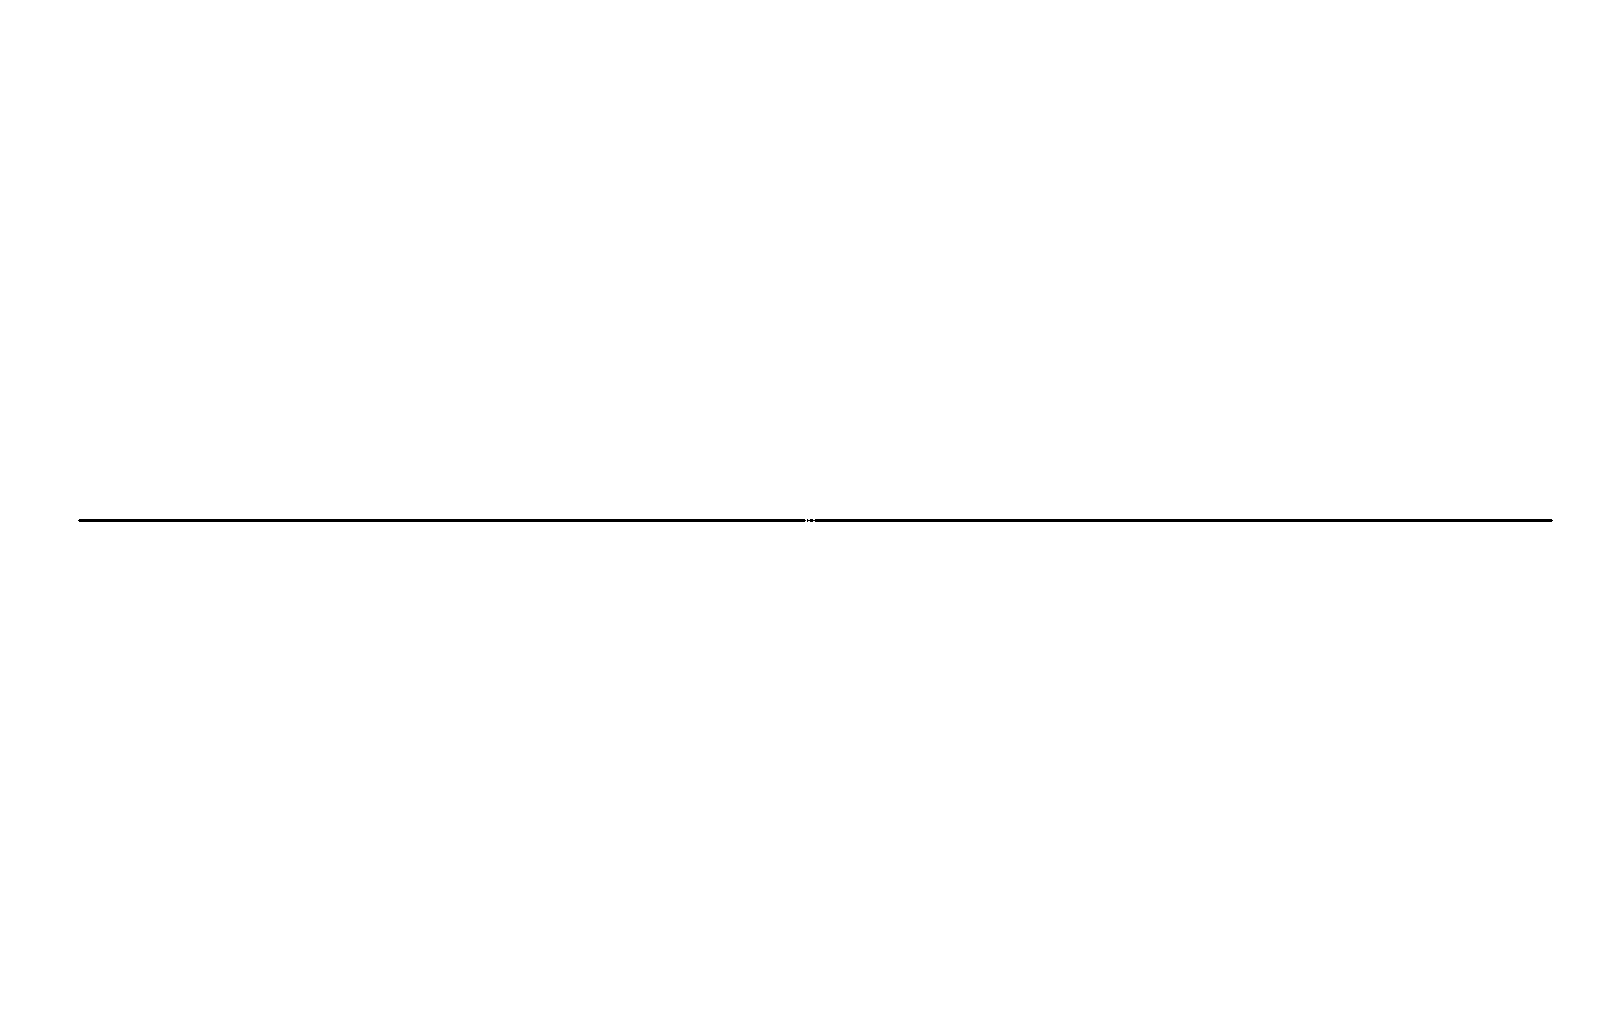
\includegraphics[width = 5 in]{2.png}
  \caption{
Example of an anisotropic emitter.
Here $D = 2.001$. 
The emitter is practically circular. 
This figure shows the circle edge-on, which is why it looks like a straight line.
The strength of the gravitational field is like $Gc$, and the intersection count gradient falloff is related to $1/r^2$.
}
\end{figure}













\begin{figure} 
\centering
  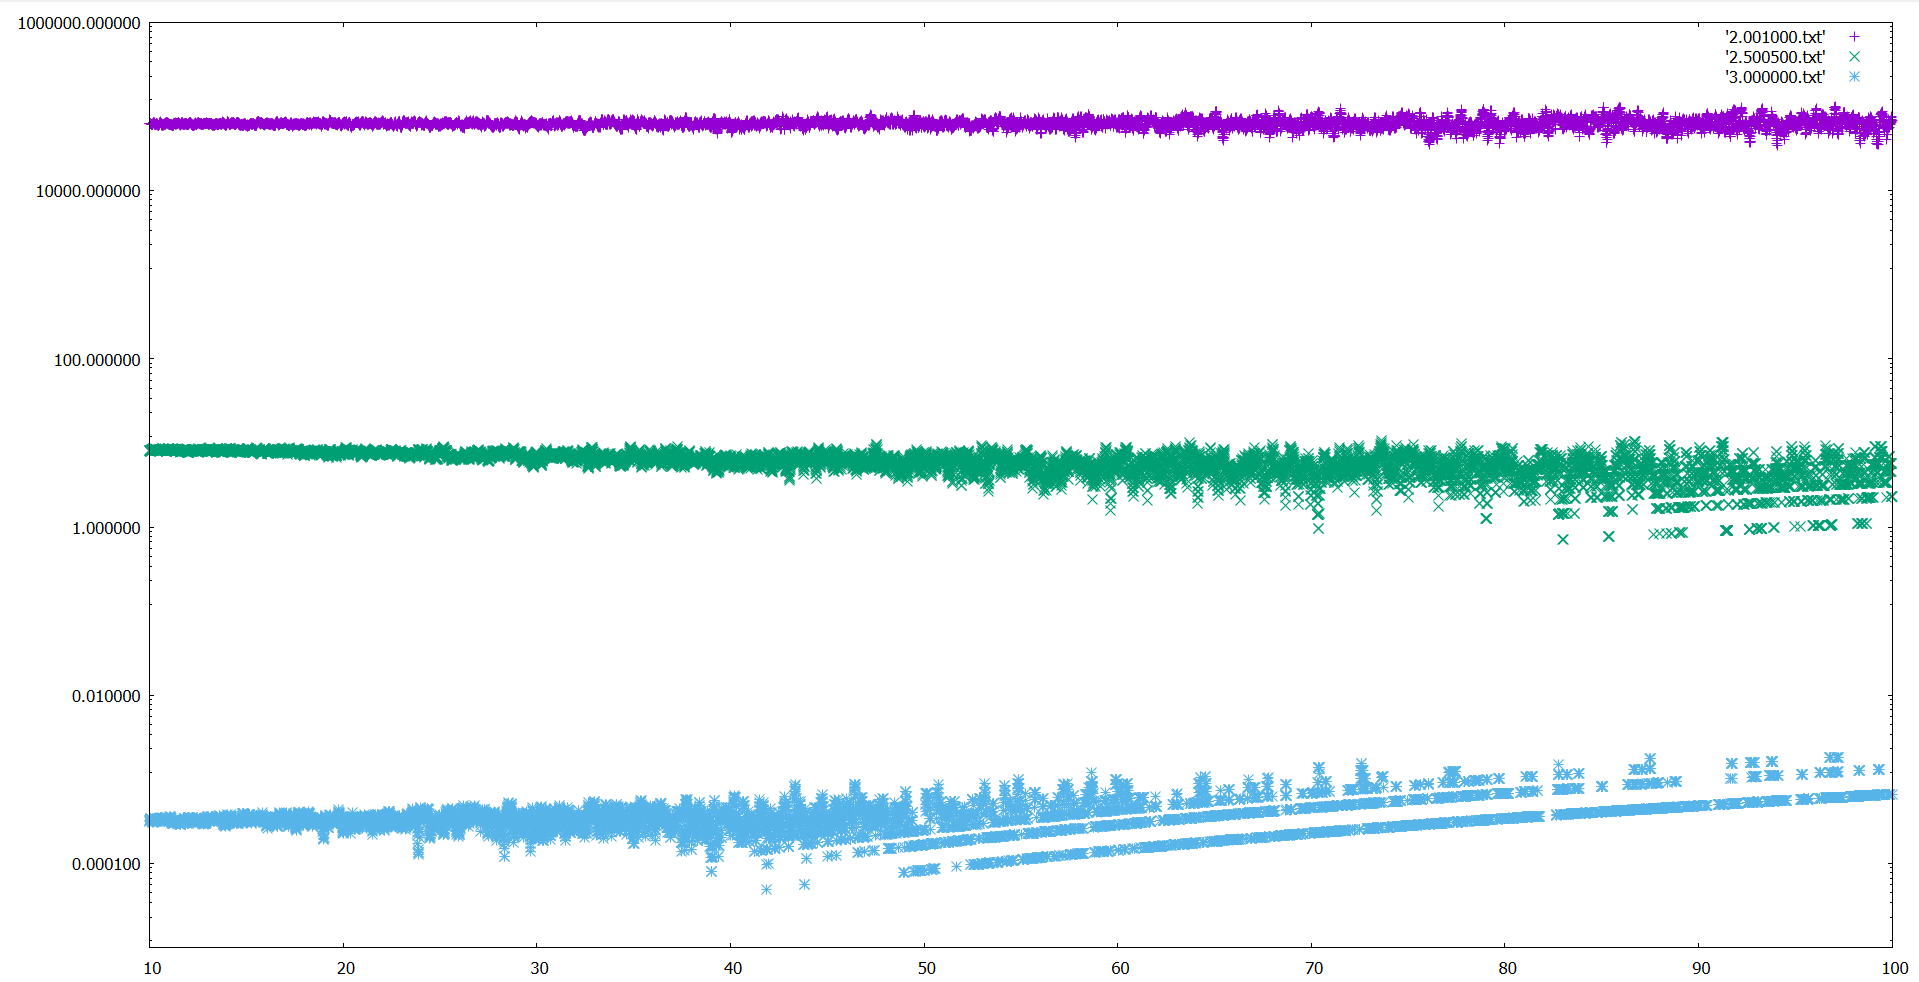
\includegraphics[width = 6 in]{multi_plot.png}
  \caption{
The $x$ axis is distance $r$, and the $y$ axis (log scaled) are the intersection count gradient times the inverse falloffs $GM c^{1} r^2$, $GM c^{0.5} r^{2.5}$, and $GM c^0 r^3$, respectively.
The banding (especially noticeable at large distance, especially where $D = 3.0$) occurs due to a relatively small oscillator count $n$ (e.g. $100,000,000$).
}
\end{figure}


\pagebreak



\begin{figure} 
\centering
  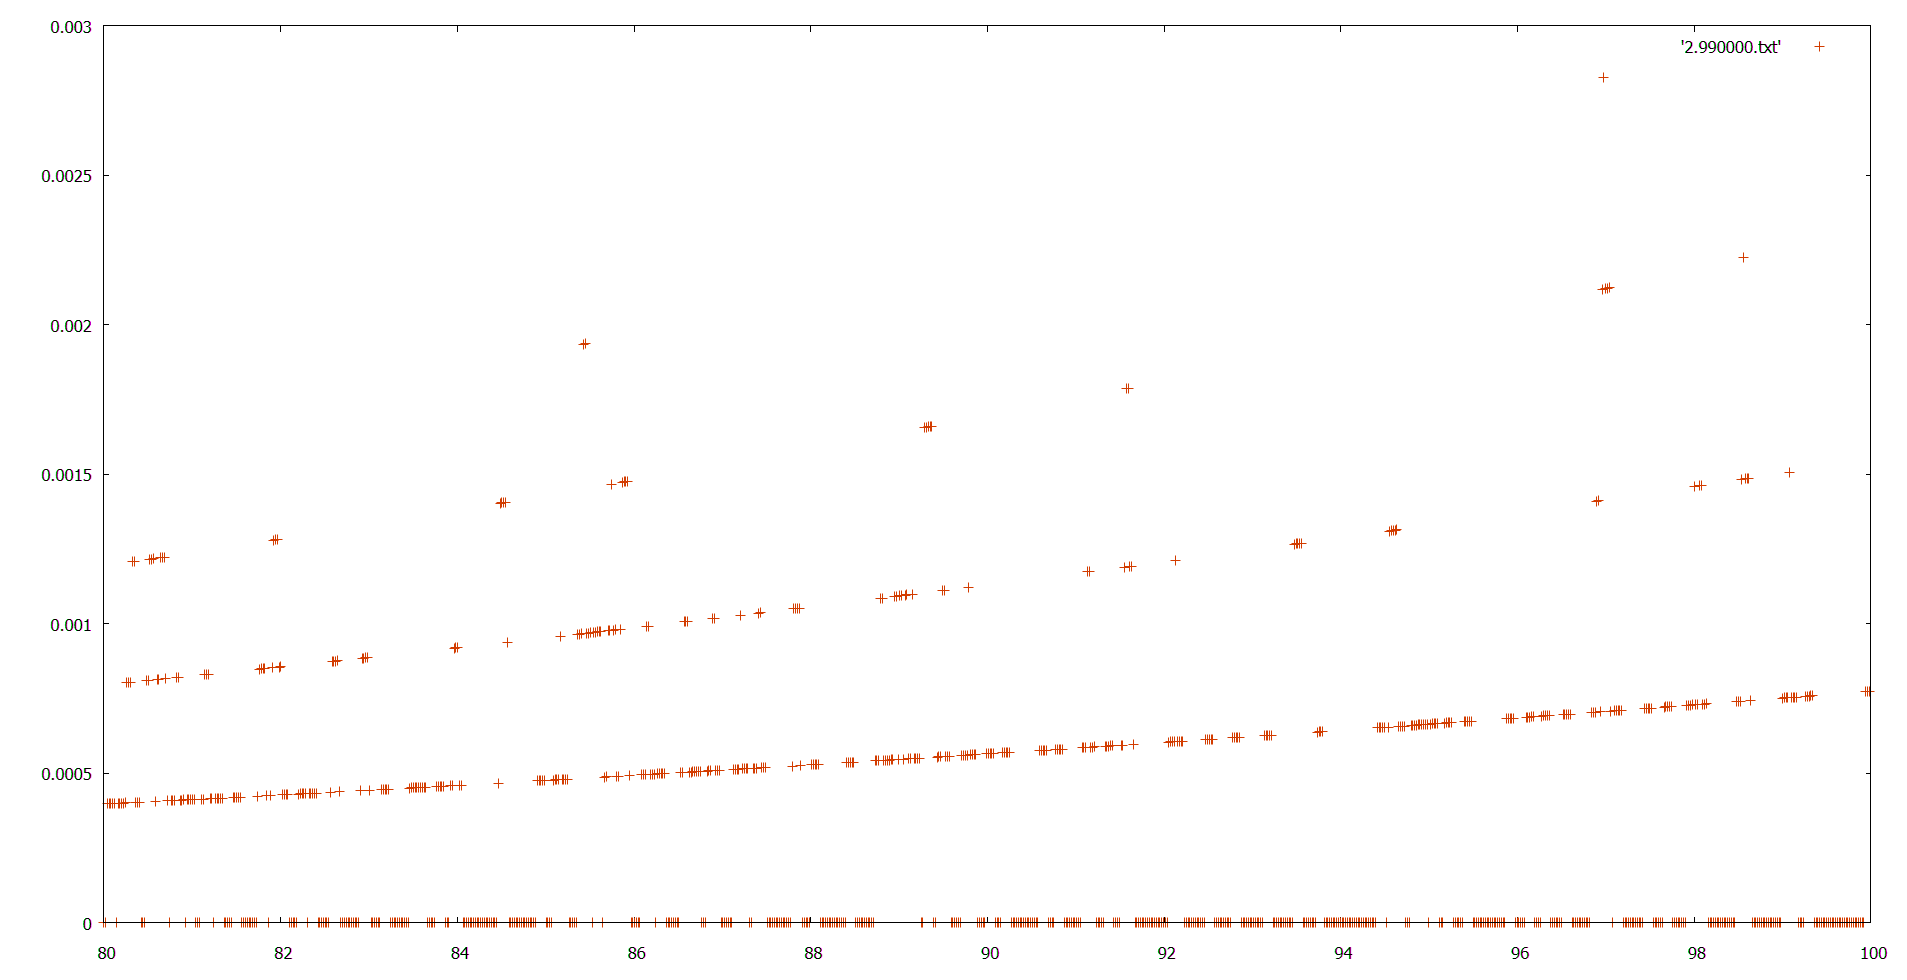
\includegraphics[width = 6 in]{10000000.png}
  \caption{
Demonstration of banding.
The $x$ axis is distance $r$, and the $y$ axis (not log scaled) is the intersection count gradient times $GM c^0 r^3$, where $D = 3.0$. $n = 10,000,000$.
}
\end{figure}


\begin{figure} 
\centering
  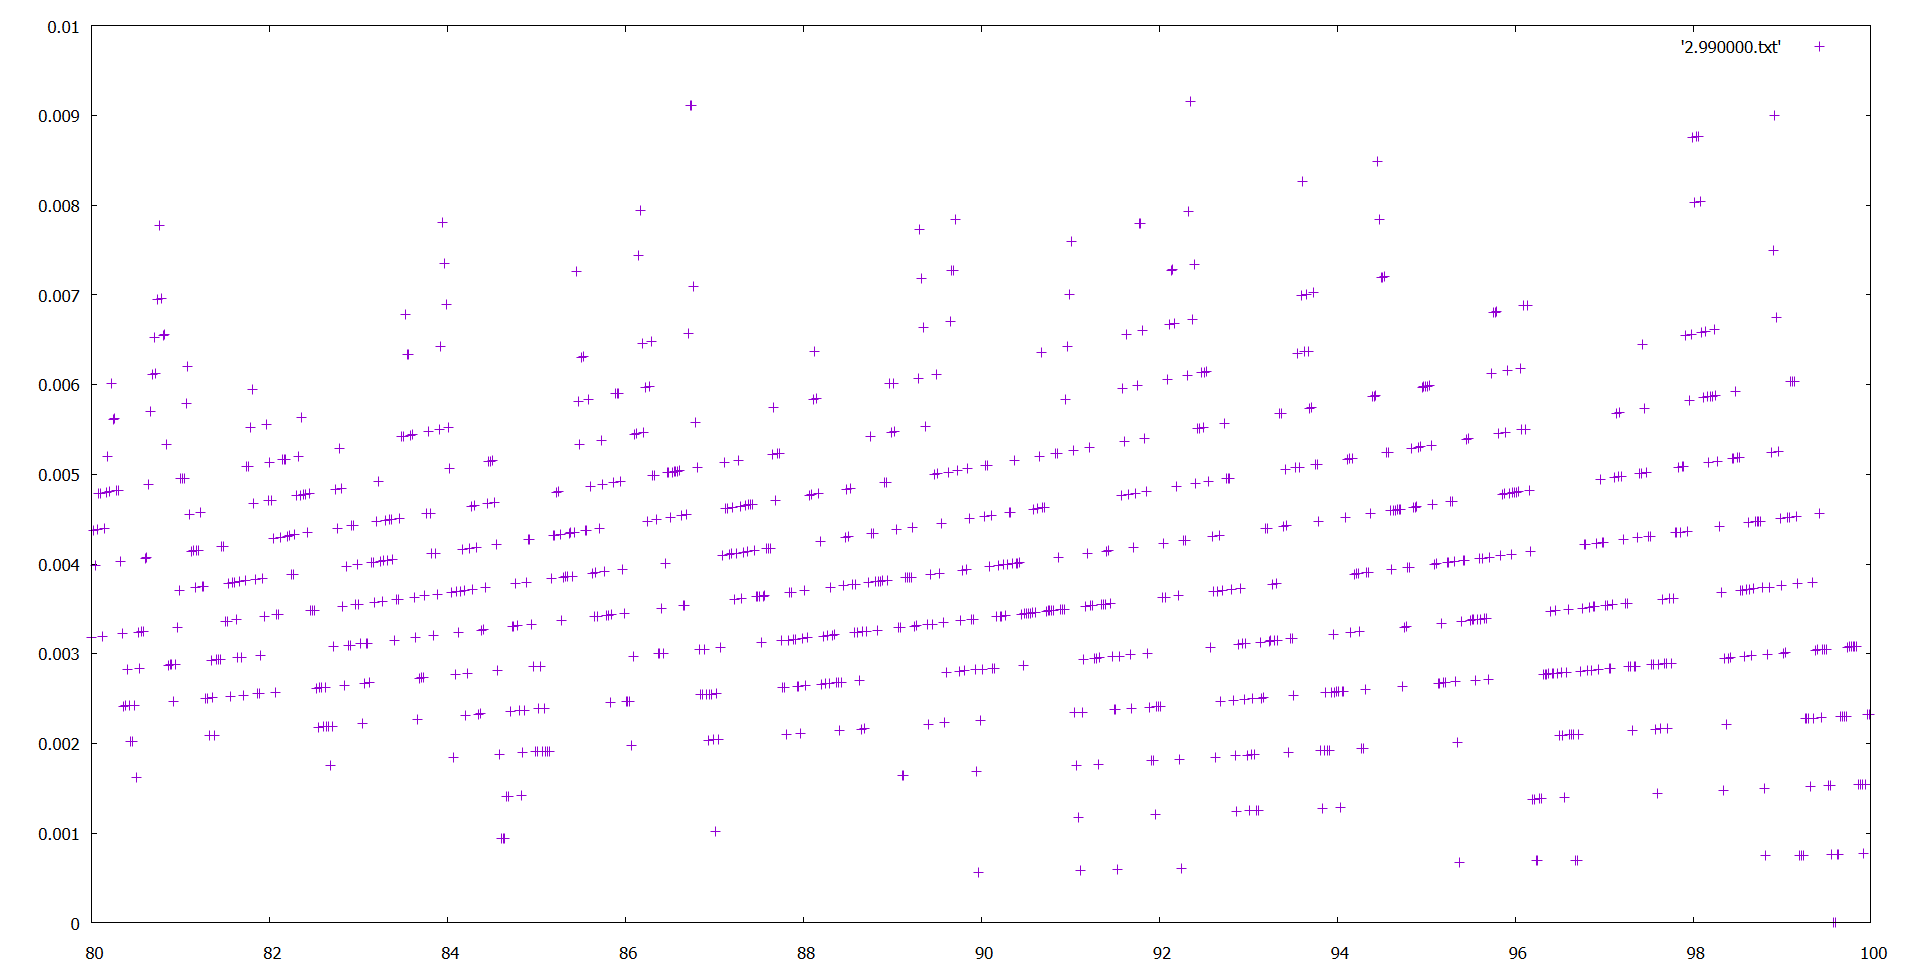
\includegraphics[width = 6 in]{100000000.png}
  \caption{
Demonstration of banding.
The $x$ axis is distance $r$, and the $y$ axis (not log scaled) is the intersection count gradient times $GM c^0 r^3$, where $D = 3.0$. $n = 100,000,000$.
The greater the number of oscillators $n$, the greater the number of bands.
}
\end{figure}




\end{document}









